\documentclass{article}
\usepackage[utf8]{inputenc}
\usepackage{authblk}
\usepackage{setspace}
\usepackage[margin=1.25in]{geometry}
\usepackage{graphicx}
\usepackage{xcolor}
\usepackage{float}
\graphicspath{ {./figures/} }
\usepackage{amsmath,amssymb,amsfonts}
\usepackage{booktabs}
\usepackage{natbib}
\usepackage{hyperref}
\hypersetup{colorlinks=true, linkcolor=blue, citecolor=blue, urlcolor=blue}

\title{\textbf{Earnings Filings and Price Reactions: An Event Study of SEC 8-K Item 2.02 Announcements for US Mega-Caps}}
\author[1]{SIQuant Research}
\affil[1]{Hypothesis $\times$ Quant}
\date{\today}
\onehalfspacing

\begin{document}
\maketitle

\begin{abstract}
\noindent \textbf{Hypothesis:} $H_0$: mean $|$CAR$[0,+1]|$ on 8-K Item 2.02 filing days equals that of ordinary days; $H_1$: it is larger \\
\textbf{Data:} 1,318 Item 2.02 filings by 35 US mega-caps, 2017-10-24 to 2026-10-22, with EDGAR acceptance timestamps \\
\textbf{Method:} Market-model abnormal returns (S\&P 500, estimation window $[-250,-31]$), reaction day set by the acceptance time in US/Eastern, 5,000-draw placebo over non-event sessions of the same stock \\
\textbf{Results:} Mean $|$CAR$|$ 4.59\% versus placebo 1.70\% (one-sided $p=0.0002$); signed mean CAR 0.059\% ($t=0.34$). \\
\textbf{Research decision:} \colorbox[rgb]{0.10,0.50,0.20}{\textcolor{white}{\textbf{\,ACCEPTED\,}}}
\end{abstract}

\section{Design}
Events come from the SEC submissions API: Form 8-K filings whose items include 2.02. A filing accepted at or after 16:00 US/Eastern (or on a non-trading day) is assigned to the next session so that the measured reaction cannot precede the disclosure \citep{mackinlay1997event}. The two-day CAR starts on that session. The placebo preserves each stock's own volatility regime.

\section{Results}
\begin{table}[h!]
\centering
\caption{Mean $|$CAR$[0,+1]|$ of Item 2.02 filings by year}
\begin{tabular}{lcc}
\toprule
Year & Events & Mean $|$CAR$|$ \\
\midrule
2017 & 24 & 4.67\% \\
2018 & 145 & 4.71\% \\
2019 & 146 & 3.98\% \\
2020 & 145 & 4.54\% \\
2021 & 142 & 3.74\% \\
2022 & 148 & 4.98\% \\
2023 & 150 & 4.41\% \\
2024 & 149 & 5.01\% \\
2025 & 145 & 4.53\% \\
2026 & 124 & 5.46\% \\
\bottomrule
\end{tabular}
\end{table}


\begin{figure}[H]
\centering
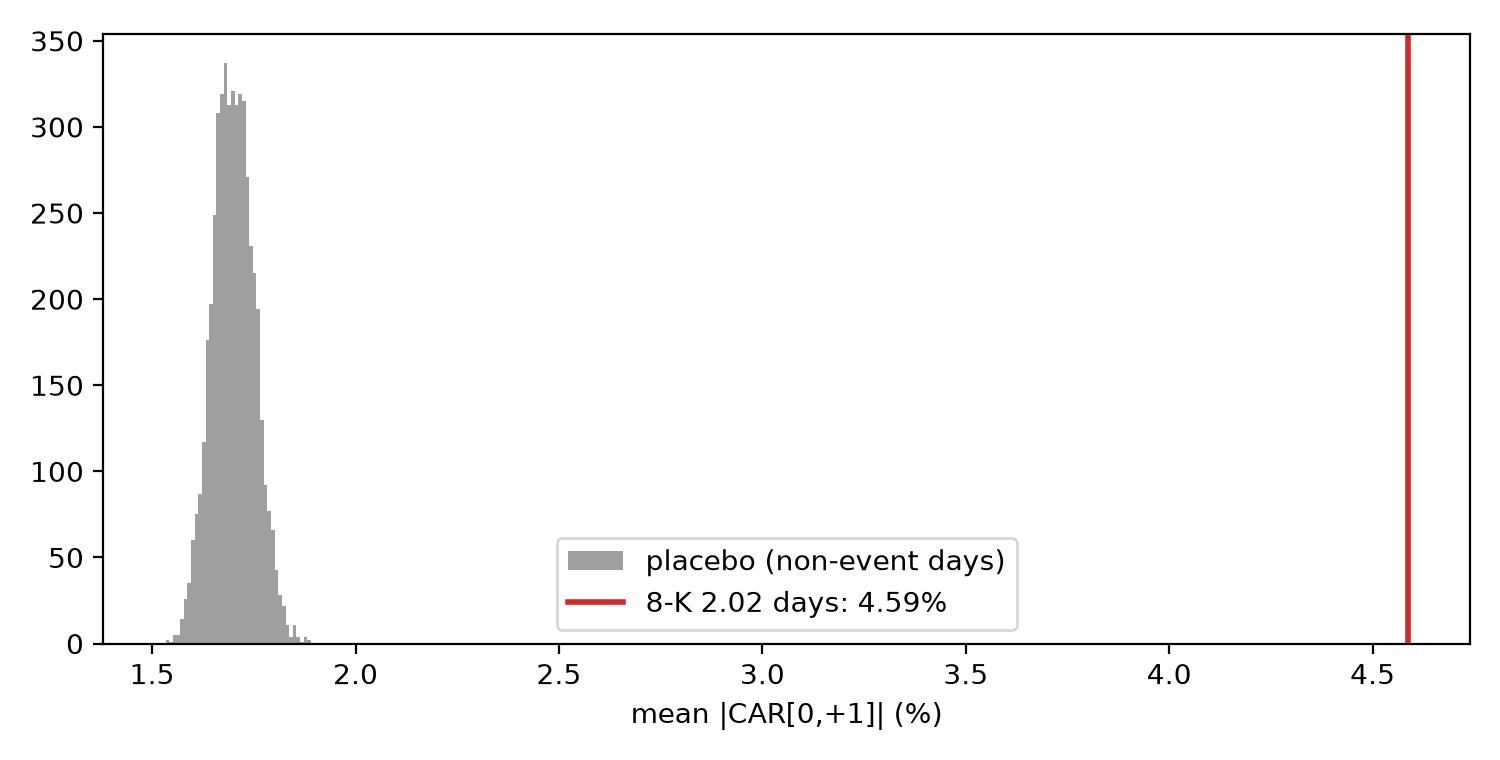
\includegraphics[width=0.8\textwidth]{fig1_earnings_car_placebo.png}
\caption{Observed mean absolute CAR against the placebo distribution.}
\end{figure}

\section{Limitations}
Filings accepted during trading hours include a pre-announcement part of the day, which understates the reaction. Earnings dates are not exogenous to volatility. The universe is today's mega-caps, so the results do not generalise to small or delisted firms. The signed CAR needs a surprise measure (consensus data is not free) and is reported only descriptively.


\bibliographystyle{plainnat}
\bibliography{references}

\end{document}
